\documentclass[12pt]{article}

\usepackage{tikz}
\usetikzlibrary{plotmarks}
\begin{document}

% PGF/TikZ picture from SSJ: Distribution of positive discounted payoff
% XScale = 1.0,  YScale = 0.01,  XShift = 0.0,  YShift = 0.0
% Therefore, thisFileXValue = (originalSeriesXValue+XShift)*XScale
%        and thisFileYValue = (originalSeriesYValue+YShift)*YScale

\begin{figure}
\begin{center}
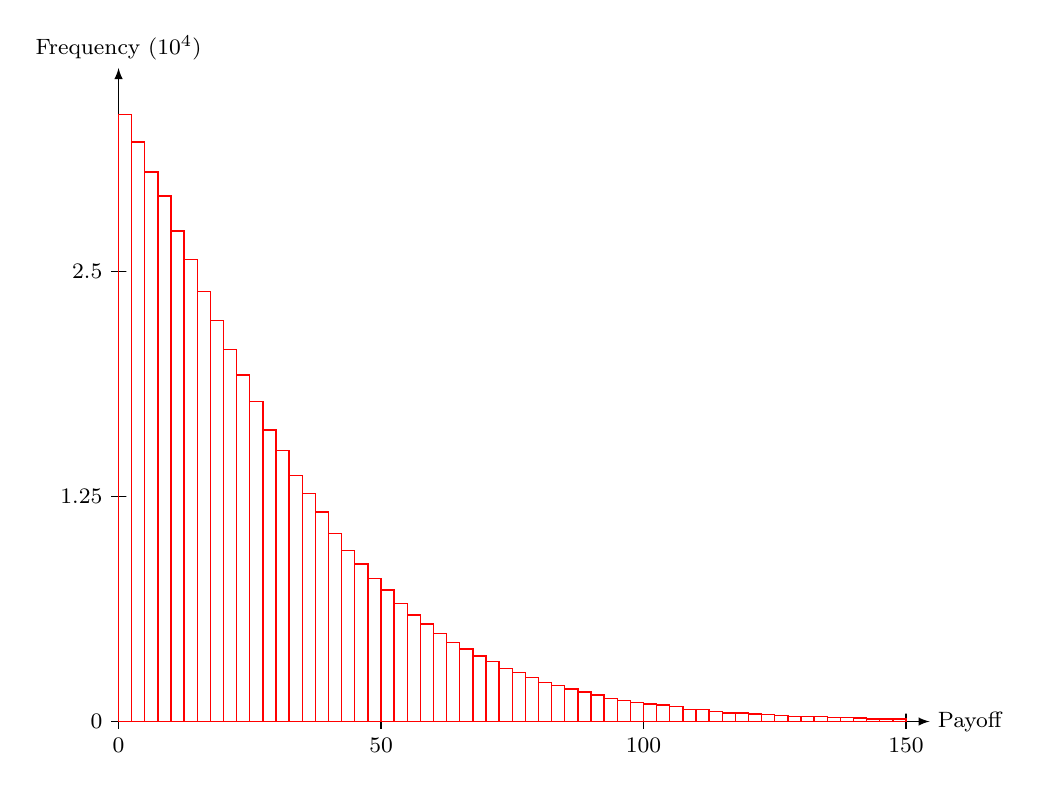
\begin{tikzpicture}[x=0.06666666666666667cm, y=0.022857142857142857cm]
\footnotesize
\draw [-latex] ([xshift=-0mm] 0.0,0) -- ([xshift=3mm] 150.0,0) node[right] {Payoff};
\draw (0.0,0) -- +(0mm,1mm) -- +(0mm,-1mm) node[below] {0};
\draw (50.0,0) -- +(0mm,1mm) -- +(0mm,-1mm) node[below] {50};
\draw (100.0,0) -- +(0mm,1mm) -- +(0mm,-1mm) node[below] {100};
\draw (150.0,0) -- +(0mm,1mm) -- +(0mm,-1mm) node[below] {150};
\draw [-latex] ([yshift=-0mm] 0,0.0) -- ([yshift=3mm] 0, 350.0) node[above] {Frequency $(10^{4})$};
\draw (0,0.0) -- +(1mm,0mm) -- +(-1mm,0mm) node[left] {0};
\draw (0,125.0) -- +(1mm,0mm) -- +(-1mm,0mm) node[left] {1.25};
\draw (0,250.0) -- +(1mm,0mm) -- +(-1mm,0mm) node[left] {2.5};
\draw [line width=0.50pt, color=red] ([xshift=0.0000] 0.0000, 0.0000) rectangle ([xshift=-0.0000] 2.5000, 337.3000); %
\draw [line width=0.50pt, color=red] ([xshift=0.0000] 2.5000, 0.0000) rectangle ([xshift=-0.0000] 5.0000, 321.9400); %
\draw [line width=0.50pt, color=red] ([xshift=0.0000] 5.0000, 0.0000) rectangle ([xshift=-0.0000] 7.5000, 305.2300); %
\draw [line width=0.50pt, color=red] ([xshift=0.0000] 7.5000, 0.0000) rectangle ([xshift=-0.0000] 10.0000, 291.9700); %
\draw [line width=0.50pt, color=red] ([xshift=0.0000] 10.0000, 0.0000) rectangle ([xshift=-0.0000] 12.5000, 272.6000); %
\draw [line width=0.50pt, color=red] ([xshift=0.0000] 12.5000, 0.0000) rectangle ([xshift=-0.0000] 15.0000, 256.8300); %
\draw [line width=0.50pt, color=red] ([xshift=0.0000] 15.0000, 0.0000) rectangle ([xshift=-0.0000] 17.5000, 238.7600); %
\draw [line width=0.50pt, color=red] ([xshift=0.0000] 17.5000, 0.0000) rectangle ([xshift=-0.0000] 20.0000, 222.7200); %
\draw [line width=0.50pt, color=red] ([xshift=0.0000] 20.0000, 0.0000) rectangle ([xshift=-0.0000] 22.5000, 206.6500); %
\draw [line width=0.50pt, color=red] ([xshift=0.0000] 22.5000, 0.0000) rectangle ([xshift=-0.0000] 25.0000, 192.6300); %
\draw [line width=0.50pt, color=red] ([xshift=0.0000] 25.0000, 0.0000) rectangle ([xshift=-0.0000] 27.5000, 177.9500); %
\draw [line width=0.50pt, color=red] ([xshift=0.0000] 27.5000, 0.0000) rectangle ([xshift=-0.0000] 30.0000, 161.8700); %
\draw [line width=0.50pt, color=red] ([xshift=0.0000] 30.0000, 0.0000) rectangle ([xshift=-0.0000] 32.5000, 150.6000); %
\draw [line width=0.50pt, color=red] ([xshift=0.0000] 32.5000, 0.0000) rectangle ([xshift=-0.0000] 35.0000, 136.5300); %
\draw [line width=0.50pt, color=red] ([xshift=0.0000] 35.0000, 0.0000) rectangle ([xshift=-0.0000] 37.5000, 126.7000); %
\draw [line width=0.50pt, color=red] ([xshift=0.0000] 37.5000, 0.0000) rectangle ([xshift=-0.0000] 40.0000, 116.3500); %
\draw [line width=0.50pt, color=red] ([xshift=0.0000] 40.0000, 0.0000) rectangle ([xshift=-0.0000] 42.5000, 104.4300); %
\draw [line width=0.50pt, color=red] ([xshift=0.0000] 42.5000, 0.0000) rectangle ([xshift=-0.0000] 45.0000, 95.0300); %
\draw [line width=0.50pt, color=red] ([xshift=0.0000] 45.0000, 0.0000) rectangle ([xshift=-0.0000] 47.5000, 87.4200); %
\draw [line width=0.50pt, color=red] ([xshift=0.0000] 47.5000, 0.0000) rectangle ([xshift=-0.0000] 50.0000, 79.5900); %
\draw [line width=0.50pt, color=red] ([xshift=0.0000] 50.0000, 0.0000) rectangle ([xshift=-0.0000] 52.5000, 73.0100); %
\draw [line width=0.50pt, color=red] ([xshift=0.0000] 52.5000, 0.0000) rectangle ([xshift=-0.0000] 55.0000, 65.5800); %
\draw [line width=0.50pt, color=red] ([xshift=0.0000] 55.0000, 0.0000) rectangle ([xshift=-0.0000] 57.5000, 59.1300); %
\draw [line width=0.50pt, color=red] ([xshift=0.0000] 57.5000, 0.0000) rectangle ([xshift=-0.0000] 60.0000, 54.2800); %
\draw [line width=0.50pt, color=red] ([xshift=0.0000] 60.0000, 0.0000) rectangle ([xshift=-0.0000] 62.5000, 49.0600); %
\draw [line width=0.50pt, color=red] ([xshift=0.0000] 62.5000, 0.0000) rectangle ([xshift=-0.0000] 65.0000, 43.9500); %
\draw [line width=0.50pt, color=red] ([xshift=0.0000] 65.0000, 0.0000) rectangle ([xshift=-0.0000] 67.5000, 40.2800); %
\draw [line width=0.50pt, color=red] ([xshift=0.0000] 67.5000, 0.0000) rectangle ([xshift=-0.0000] 70.0000, 36.3800); %
\draw [line width=0.50pt, color=red] ([xshift=0.0000] 70.0000, 0.0000) rectangle ([xshift=-0.0000] 72.5000, 33.4800); %
\draw [line width=0.50pt, color=red] ([xshift=0.0000] 72.5000, 0.0000) rectangle ([xshift=-0.0000] 75.0000, 29.5600); %
\draw [line width=0.50pt, color=red] ([xshift=0.0000] 75.0000, 0.0000) rectangle ([xshift=-0.0000] 77.5000, 27.0700); %
\draw [line width=0.50pt, color=red] ([xshift=0.0000] 77.5000, 0.0000) rectangle ([xshift=-0.0000] 80.0000, 24.3800); %
\draw [line width=0.50pt, color=red] ([xshift=0.0000] 80.0000, 0.0000) rectangle ([xshift=-0.0000] 82.5000, 21.7800); %
\draw [line width=0.50pt, color=red] ([xshift=0.0000] 82.5000, 0.0000) rectangle ([xshift=-0.0000] 85.0000, 20.0200); %
\draw [line width=0.50pt, color=red] ([xshift=0.0000] 85.0000, 0.0000) rectangle ([xshift=-0.0000] 87.5000, 18.1700); %
\draw [line width=0.50pt, color=red] ([xshift=0.0000] 87.5000, 0.0000) rectangle ([xshift=-0.0000] 90.0000, 16.3200); %
\draw [line width=0.50pt, color=red] ([xshift=0.0000] 90.0000, 0.0000) rectangle ([xshift=-0.0000] 92.5000, 14.6400); %
\draw [line width=0.50pt, color=red] ([xshift=0.0000] 92.5000, 0.0000) rectangle ([xshift=-0.0000] 95.0000, 12.8700); %
\draw [line width=0.50pt, color=red] ([xshift=0.0000] 95.0000, 0.0000) rectangle ([xshift=-0.0000] 97.5000, 11.7800); %
\draw [line width=0.50pt, color=red] ([xshift=0.0000] 97.5000, 0.0000) rectangle ([xshift=-0.0000] 100.0000, 10.5800); %
\draw [line width=0.50pt, color=red] ([xshift=0.0000] 100.0000, 0.0000) rectangle ([xshift=-0.0000] 102.5000, 9.7300); %
\draw [line width=0.50pt, color=red] ([xshift=0.0000] 102.5000, 0.0000) rectangle ([xshift=-0.0000] 105.0000, 9.1400); %
\draw [line width=0.50pt, color=red] ([xshift=0.0000] 105.0000, 0.0000) rectangle ([xshift=-0.0000] 107.5000, 8.2900); %
\draw [line width=0.50pt, color=red] ([xshift=0.0000] 107.5000, 0.0000) rectangle ([xshift=-0.0000] 110.0000, 6.8000); %
\draw [line width=0.50pt, color=red] ([xshift=0.0000] 110.0000, 0.0000) rectangle ([xshift=-0.0000] 112.5000, 6.6300); %
\draw [line width=0.50pt, color=red] ([xshift=0.0000] 112.5000, 0.0000) rectangle ([xshift=-0.0000] 115.0000, 5.4700); %
\draw [line width=0.50pt, color=red] ([xshift=0.0000] 115.0000, 0.0000) rectangle ([xshift=-0.0000] 117.5000, 4.7700); %
\draw [line width=0.50pt, color=red] ([xshift=0.0000] 117.5000, 0.0000) rectangle ([xshift=-0.0000] 120.0000, 4.6700); %
\draw [line width=0.50pt, color=red] ([xshift=0.0000] 120.0000, 0.0000) rectangle ([xshift=-0.0000] 122.5000, 4.2700); %
\draw [line width=0.50pt, color=red] ([xshift=0.0000] 122.5000, 0.0000) rectangle ([xshift=-0.0000] 125.0000, 3.9300); %
\draw [line width=0.50pt, color=red] ([xshift=0.0000] 125.0000, 0.0000) rectangle ([xshift=-0.0000] 127.5000, 3.4500); %
\draw [line width=0.50pt, color=red] ([xshift=0.0000] 127.5000, 0.0000) rectangle ([xshift=-0.0000] 130.0000, 2.8200); %
\draw [line width=0.50pt, color=red] ([xshift=0.0000] 130.0000, 0.0000) rectangle ([xshift=-0.0000] 132.5000, 2.7600); %
\draw [line width=0.50pt, color=red] ([xshift=0.0000] 132.5000, 0.0000) rectangle ([xshift=-0.0000] 135.0000, 2.6200); %
\draw [line width=0.50pt, color=red] ([xshift=0.0000] 135.0000, 0.0000) rectangle ([xshift=-0.0000] 137.5000, 2.3300); %
\draw [line width=0.50pt, color=red] ([xshift=0.0000] 137.5000, 0.0000) rectangle ([xshift=-0.0000] 140.0000, 2.2500); %
\draw [line width=0.50pt, color=red] ([xshift=0.0000] 140.0000, 0.0000) rectangle ([xshift=-0.0000] 142.5000, 1.9700); %
\draw [line width=0.50pt, color=red] ([xshift=0.0000] 142.5000, 0.0000) rectangle ([xshift=-0.0000] 145.0000, 1.5000); %
\draw [line width=0.50pt, color=red] ([xshift=0.0000] 145.0000, 0.0000) rectangle ([xshift=-0.0000] 147.5000, 1.4900); %
\draw [line width=0.50pt, color=red] ([xshift=0.0000] 147.5000, 0.0000) rectangle ([xshift=-0.0000] 150.0000, 1.3100); %
\end{tikzpicture}
\end{center}
\caption{Distribution of positive discounted payoff}
\end{figure}
\end{document}
